\section{Architektur}

\begin{figure}[ht!]
	\centering
	\begin{center}
	  \makebox[\textwidth]{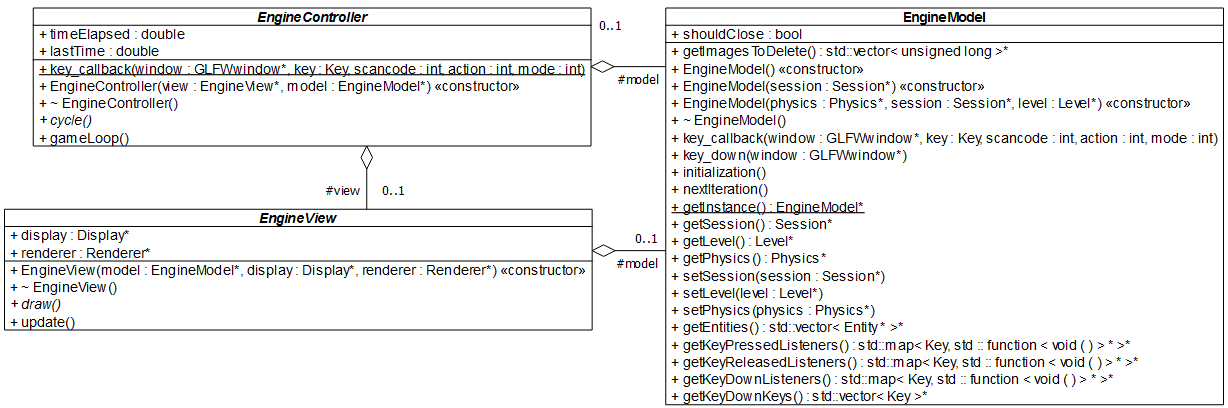
\includegraphics[width=450pt]{images/mvc_cd}}
	\end{center}
     \caption{Ein Klassendiagramm, welches die Beziehungen zwischen Model, View und Controller darstellen soll.}
     \label{fig:class_diagram:mvc}
\end{figure}

Die Architektur des Rahmenwerks folgt dem Entwicklungsmuster MVC - Model View Controller. Dabei wird das Rahmenwerk in 3 Aufgabenbereiche aufgespalten:
\begin{enumerate}
\item Der \textbf{Controller} (hier \textbf{EngineController} genannt) kontrolliert den Programmfluss, indem er auf Benutzereingaben wartet und auf diese mit  Weiterleitungen auf die entsprechenden Programmmethoden reagiert.
\item Die \textbf{View} (hier \textbf{EngineView} genannt) stellt den aktuellen Programmzustand auf dem Bildschirm dar.
\item Das \textbf{Model} (hier \textbf{EngineModel} genannt) stellt alle Logik-relevanten Programmmethoden und das Datenmodell bereit.
\end{enumerate}
Kommunikation zwischen den genannten Komponenten darf ohne weiteres nur von Controller zu View, von Controller zu Model und von View zu Model erfolgen.
Kommunikation von Model zu View und View zu Controller sind nur gestattet durch Anwendung des Observer-Entwicklungsmusters. Dies beugt unter Anderem der Entstehung zyklischer Abhängigkeiten im Programm vor und steigert somit die Freundlichkeit gegenüber den Nutzern des Rahmenwerks.